\documentclass{article}
\usepackage{graphicx,amsmath,mdframed,amsfonts,amssymb, inputenc}


\newmdtheoremenv{law}{Law}

\title{Computation \& Robot Vision: Lecture 2, Camera parameters}
\author{Sam Barrett}

\begin{document}
\maketitle

Digital images are fundamentally \textbf{spatially discrete}, meaning they are divided up into a countable number of subsections. Usually, these subsections take the form of rectangular picture elements or \textit{pixels}.

\textbf{Note:} the perspective equation derived in the previous lecture is only valid when all distances are measured from the camera's reference frame and when image coordinates have their origin at the image centre, where the axis of symmetry of the camera pierces the retina or sensor.

In practice, the world and camera coordinate systems are related by a set of physical parameters including:

\begin{itemize}
  \item The focal length $f$ of the the lens
  \item the size of the individual pixels on the sensor.
  \item the position of the image centre
  \item the position and orientation of the camera.
\end{itemize}

There are a number of issues with this system however, including that one unit in the camera's coordinate system may not be the same as one unit in the world coordinate system (resulting in perspective shift or objects appearing relatively larger than they actually are). This is related to what is known as the \textbf{intrinsic parameter problem} where intrinsic parameters include focal length, principal point, aspect ratio and the angle between the axis.

Another issue is that a cameras coordinate system will have a different position and rotation in space to that of the world. This is related to the \textbf{extrinsic parameter problem}

\[
  \begin{pmatrix}
    U \\ V \\ W
  \end{pmatrix} =
  \overbrace{\begin{pmatrix}
    1&0&0&0\\
    0&1&0&0\\
    0&0&1&0\\
  \end{pmatrix}}^{\text{transformation representing intrinsic parameters}}
\cdot
  \underbrace{\begin{pmatrix}
    X \\ Y \\ Z \\ T
  \end{pmatrix}}_{\text{transformation representing extrinsic parameters}}
\]


\section{Single-view geometry}
\label{sec:singleview}

Here we work with a single camera. Imagine there is one point in a world 3D coordinate system (c.s.), $P$. Our 3D c.s. has some origin $O$, so we can now represent $P$ in the world with a set of coordinates relative to $O$. We want now to project $P$ onto the image plane, the image plane is located in the camera 3D c.s., which is separate from the world c.s.. We can have two different kinds of projection:

\begin{enumerate}
  \item ``Extrinsic'' projection: the 3D world coordinate system should be projected onto the 3D camera coordinate system
  \item ``Intrinsic'' projection: the 3D camera coordinate system should be projected onto the 2D image plane.
\end{enumerate}

\subsection{Intrinsic projection}
\label{subsec:intrinsic-projection}

The steps of an intrinsic projection are as follows:

\begin{itemize}
  \item Given a point $P$ in the camera 3D coordinate system which is measured in \textbf{metres}
  \item We project $P$ onto the camera image plane, also measured in \textbf{metres}
  \item We then project from our 2D image plane to a discretisesd image which is measured in \textbf{pixels}
\end{itemize}

\subsubsection{Homogeneous coordinates}

Euclidean geometry uses the \textbf{Cartesian coordinates system}, however, for a projective geometry, \textbf{homogeneous coordinates} are more appropriate.

Conversion is simple: add an extra element at the \textit{'end'}:

\[
  \overbrace{\begin{bmatrix}
      x \\y
    \end{bmatrix}}^{\text{Cartesian form}}
  \rightarrow
  \overbrace{\begin{bmatrix}
      x \\y \\ 1
    \end{bmatrix}}^{\text{Homogeneous form}}
\]

This system has the benefit that if a point is multiplied by a non-zero scalar value $w$, our point does not change:

\[
  \begin{bmatrix}
    x \\ y\\ 1
  \end{bmatrix} \equiv
  \begin{bmatrix}
    wx \\ wy \\ w
  \end{bmatrix}
\]

In order to convert from a homogeneous to a Euclidean system: divide by the last coordinate to make it equal to 1 and ignore it.


\subsubsection{Concepts}

\begin{itemize}
  \item Principal axis: this is a line from the camera centre perpendicular to the image plane.
  \item Principal point: this is a point where the principal axis punctures the image plane
  \item Normalised camera coordinate system: this is a system with its origin at the principal point
\end{itemize}

\subsubsection{Pinhole camera: revisited}

With our new coordinate system, we can now revisit the pinhole camera from the previous lecture.

A 3D point in the world coordinate system can be mapped to a 2D projection in the image plane as follows:

\[
  \begin{bmatrix}
    X \\ Y \\ Z \\ 1
  \end{bmatrix} \mapsto
  \begin{bmatrix}
    f \frac{X}{Z} \\ f \frac{Y}{Z} \\ 1
  \end{bmatrix}
\]

This can be represented as a vector-matrix multiplication:

\[
  \overbrace{\begin{pmatrix}
    f X \\ f Y \\ Z
  \end{pmatrix}}^{\bf x} =
  \underbrace{\begin{bmatrix}
    f & & & 0\\
    & f & & 0\\
    & & 1 & 0\\
  \end{bmatrix}}_{\bf P_{0}}
  \overbrace{\begin{pmatrix}
X \\Y \\ Z \\ 1
\end{pmatrix}}^{\bf X}
\]

which can also be written
\[
  \bf x = P_{0}X
\]

We can re-write the projection matrix $\bf P_{0}$ to separate the focal lengths:

\[
  \mathbf{P_{0}} = \text{diag}([f,f,1])[\text{I}|0] = \begin{bmatrix}
    f & & \\
    & f & \\
    & & 1 \\
  \end{bmatrix}\begin{bmatrix}
    1 & & & 0 \\
    & 1 & & 0 \\
    & & 1 & 0 \\
  \end{bmatrix}
\]

\subsubsection{Image plane to image pixels}

\begin{itemize}
  \item Our normalised camera coordinate system has it's origin at the principal point $p = [p_{x},p_{y}]^{\text{T}}$.
  \item Our image coordinate system has it's origin in the corner of the image sensor.
\end{itemize}

This can be seen in Figure~\ref{fig:1}

\begin{figure}[ht]
  \centering
  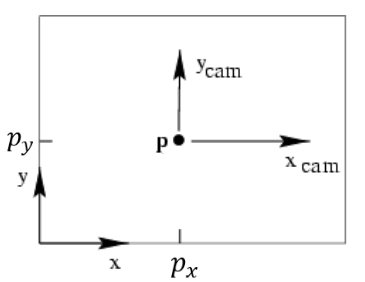
\includegraphics[scale=0.7]{figures/l2-1.png}
  \caption{\label{fig:1} Figure showing camera and image coordinate systems}
\end{figure}

Moving our camera coordinate system origin to $p$ makes our calculations much easier as we only need consider positive numbers. It allows our transformation seen above to become:

\[
  (X,Y,Z)\mapsto (f \frac{X}{Z}+p_{x}, f \frac{Y}{Z}+p_{y})
\]

Which, in vector-matrix multiplication becomes:

\[
  \begin{pmatrix}
    f X + Z p_{x} \\
    f Y + Z p_{y} \\
    Z
  \end{pmatrix} =
  \begin{bmatrix}
    f & 0 & p_{x} & 0\\
    0 & f & p_{y} & 0\\
    0 & 0 & 1 & 0
  \end{bmatrix}
  \begin{pmatrix}
    X \\ Y \\ Z \\ 1
  \end{pmatrix}
\]

\subsubsection{From image plane to image pixels}

We now want to project onto our sensor of size Ws $\times$ Hs (in metres). We represent pixels in a rectangular $M_{x} \times M_{y}$ matrix.

Let $m_{x} = \frac{M_{x}}{W_{s}}$ and $m_{y} = \frac{M_{y}}{H_{s}}$

We now construct the following projection in vector-matrix multiplication form:

\[
  \begin{pmatrix}
    x \\y \\z
  \end{pmatrix}
  = \underbrace{\begin{bmatrix}
    m_{x} & 0 & 0\\
    0 & m_{y} & 0\\
    0 & 0 & 1
  \end{bmatrix}}_{\text{pixel /m}}
  \underbrace{\begin{bmatrix}
    f & 0 & p_{x} & 0\\
    0 & f & p_{y} & 0\\
    0 & 0 & 1 & 0
  \end{bmatrix}}_{\text{m}}
  \begin{pmatrix}
    X \\Y\\ Z\\1
  \end{pmatrix}
\]

Which can also be written:

\[
  \begin{pmatrix}
    x \\ y \\z
  \end{pmatrix} =
  \begin{bmatrix}
    \alpha_{x} & 0  & x_{0} & 0\\
    0 & \alpha_{y} & y_{0} & 0\\
    0 & 0 & 1 & 0
  \end{bmatrix}
  \begin{pmatrix}
    X \\ Y \\ Z \\1
  \end{pmatrix}
\]

It is often difficult to guarantee a perfectly rectangular sensor, so we also have a case for a skewed sensor, here we simply add a single value to the projection matrix $\bf P_{0}$ to form:


\[
  \begin{pmatrix}
    x \\ y \\z
  \end{pmatrix} =
  \begin{bmatrix}
    \alpha_{x} & s  & x_{0} & 0\\
    0 & \alpha_{y} & y_{0} & 0\\
    0 & 0 & 1 & 0
  \end{bmatrix}
  \begin{pmatrix}
    X \\ Y \\ Z \\1
  \end{pmatrix}
\]


We can decompose $\bf P_{0}$ into two separate matrices to allow for easier computation and reasoning, we can construct $\bf P_{0}$ from the product of a square matrix $K$ and a concatination of the $3\times 3$ identity matrix and a 3D 0-vector:

\[
  \mathbf{P_{0}} = \mathbf{K}[\textbf{I}|0] = \begin{bmatrix}
    \alpha_{x} & s  & x_{0} \\
    0 & \alpha_{y} & y_{0} \\
    0 & 0 & 1
  \end{bmatrix}
  \begin{bmatrix}
    1 & 0 & 0 & 0 \\
    0 & 1 & 0 & 0 \\
    0 & 0 & 1 & 0 \\
  \end{bmatrix}
\]

We refer to $\bf K$ as our \textbf{projection matrix} which prescribes the projection of any 3D point in the camera coordinate system onto our pixels.

Where:
\begin{itemize}
  \item $\alpha_{x}= m_{x} \cdot f$
  \item $\alpha_{y} = m_{y} \cdot f$
  \item $x_{0} = p_{x} \cdot m_{x}$
  \item $y_{0} = p_{y} \cdot m_{y}$
  \item $s$ is our skewness factor
\end{itemize}



\subsection{Extrinsic Projection}
\label{subsec:extrinsic-projection}

Here we are concerned with how to project the world coordinate system onto the 3D camera coordinate system.

The 3D camera coordinate system is related to the 3D world coordinate system by a rotation matrix $\bf R$ and translation $\bf \tilde{t} = \tilde{C}$

In Euclidean terms we can write this process of translation followed by rotation as:

\[
  \tilde{X}_{\text{cam}}= \mathbf{R}(\tilde{X}-\mathbf{\tilde{C}} )
\]

Our camera is specified by a calibration matrix $\bf K$, the projection centre in the world coordinate system is given by $\bf \tilde{C}$ and a rotation matrix $\bf R$. A 3D point given in (homogeneous) world coordinates $\bf X$ is projected onto pixels $\bf x$ by the following relation:

\[
  \mathbf{x} = \mathbf{K}[\text{I}|0]\tilde{X}_{\text{cam}} = \mathbf{K} [\mathbf{R} | t]\mathbf{X} = P \mathbf{X}
\]

Where:

\begin{itemize}
  \item $P = \mathbf{K}[\mathbf{R}|t ]$
  \item $t = -\mathbf{R \tilde{C}}$
\end{itemize}

Lenses add more complexity through non-linearity, previously straight lines are no longer straight, leading to image distortion.

Lens distortion assumes radially symmetric lenses. We radially expand an image to un-distort it, here only the point changes, not the angle.

Our extrinsic parameters include camera rotation and camera translation.

\subsection{Vanishing Points}

We can now give a more robust definition of vanishing points,

If we consider a point on one of two parallel lines $l_{1}$ and $l_{2}$, $\mathbf{A} = \begin{bmatrix}
X_{A}\\Y_{A}\\Z_{A}
\end{bmatrix} $ and a vector $D$ from $A$, $D = \begin{bmatrix}
X_{D}\\ Y_{D}\\Z_{D}
\end{bmatrix}$.

A point on a the line $\mathbf{X}(\lambda) = \mathbf{A} = \lambda \mathbf{D}   $ is projected to a point $x(\lambda)$ in the image plane by:

\[
  x(\lambda) = \begin{bmatrix}
    x\\y
  \end{bmatrix} = \begin{bmatrix}
    f \frac{X}{Z}\\ f \frac{Y}{Z}
  \end{bmatrix}=
  \begin{bmatrix}
    \frac{f(X_{A} + \lambda X_{D})}{(Z_{A}+ \lambda Z_{D})}\\
    \frac{f(Y_{A}+\lambda Y_{D})}{(Z_{A}+ \lambda Z_{D})}
  \end{bmatrix}
\]

Here we can see that as $\mathbf{X}(\lambda) \rightarrow \infty $, $x(\lambda)$ tends towards the vanishing point, $\mathbf{v} $.


\[
  \mathbf{v} = \lim_{\lambda \to \infty}x(\lambda) = \lim_{\lambda \to \infty} \begin{bmatrix}
    f \frac{X_{A}+ \lambda X_{D}}{Z_{A}+ \lambda Z_{D}} \\
    f \frac{Y_{A}+ \lambda Z_{D}}{Z_{A} + \lambda Z_{D}}
  \end{bmatrix}
\]

Giving us a vanishing point of:

\[
  \mathbf{v} = \begin{bmatrix}
    f \frac{X_{D}}{Z_{D}} \\
    f \frac{Y_{D}}{Z_{D}}
  \end{bmatrix}
\]

Our vanishing point depends on the direction $\bf D$ and not on the point $\mathbf{A} $, meaning that a different set of parallel lines even if they share a point, have a different vanishing point.

\subsection{Homography}
\label{subsec:homography}

Homography is the process of projecting points or images from image plane to image plane. It has many uses from Image stitching to augmented reality.

In order to estimate the homography we must find all corresponding points between the two image planes.

Assuming we know all corresponding points between $\bf x$ and $\bf x'$ we can represent the translation as:

\[
  w \mathbf{x'} = \mathbf{Hx}
\]

Or,

\[
  w \begin{bmatrix}
    x' \\ y' \\ 1
  \end{bmatrix} =
  \begin{bmatrix}
    H_{1 1} & H_{1 2} & H_{1 3} \\
    H_{2 1} & H_{2 2} & H_{2 3} \\
    H_{3 1} & H_{3 2} & H_{3 3} \\
  \end{bmatrix}
  \begin{bmatrix}
    x \\ y \\ 1
  \end{bmatrix}
\]

Where the elements of $\bf H$ can be estimated by applying a direct linear transform or \textbf{DLT}.

For each corresponding point $i$ we have:


\[
  w \mathbf{x'_{i}} = \mathbf{Hx_{i}}
\]

\[
  w \begin{bmatrix}
    x'_{i} \\ y'_{i} \\ 1
  \end{bmatrix} =
  \begin{bmatrix}
    H_{1 1} & H_{1 2} & H_{1 3} \\
    H_{2 1} & H_{2 2} & H_{2 3} \\
    H_{3 1} & H_{3 2} & H_{3 3} \\
  \end{bmatrix}
  \begin{bmatrix}
    x_{i}\\ y_{i} \\ 1
  \end{bmatrix} =
  \begin{bmatrix}
    h_{1}^{T} \\ h_{2}^{T} \\ h_{3}^{T}
  \end{bmatrix}X_{i} = \begin{bmatrix}
    h_{1}^{T}X_{i} \\ h_{2}^{T}X_{i} \\ h_{3}^{T}X_{i}
  \end{bmatrix}
\]

As these are equal, by the definition of cross-product:

\[
  \mathbf{x'_{i}} \times \mathbf{Hx_{i}}  = 0
\]

We can rearrange this vector product into a a vector-matrix product:

\[
  \mathbf{x'_{i}} \times \begin{bmatrix}
    h_{1}^{T} x_{i}\\ h_{2}^{T}x_{i} \\ h_{3}^{T}x_{i}
  \end{bmatrix}  =
  \begin{bmatrix}
    \mathbf{x'}_{i\times}
  \end{bmatrix}\begin{bmatrix}
    x_{i}^{T}h_{1}\\ x_{i}^{T}h_{2} \\ x_{i}^{T}h_{3}
  \end{bmatrix} =
  \begin{bmatrix}
    0 & -1 & y'_{i} \\
    1 & 0 & x'_{i} \\
    -y'_{i} & x'_{i} & 0
  \end{bmatrix}\begin{bmatrix}
    x_{i}^{T}h_{1}\\ x_{i}^{T}h_{2} \\ x_{i}^{T}h_{3}
  \end{bmatrix}
\]

We can then multiply these matrix terms and expose the homography terms $h_{1}, h_{2}, h_{3}$ into a single vector:

\[
  \mathbf{x'_{i}}\times \mathbf{Hx_{i}} = \begin{bmatrix}
    0^{T} & - \mathbf{x_{i}^{T}} & y'_{i}\mathbf{x}_{i}^{T} \\
    \mathbf{x}_{i}^{T} & 0^{T} & -\mathbf{x'}_{i}\mathbf{x}_{i}^{T} \\
    -y'_{i} \mathbf{x}
  \end{bmatrix}
\]

I fucking give up, fuck this




\end{document}
